%\documentclass{beamer}
%Для защит онлайн лучше использовать разрешение 16x9
\documentclass[aspectratio=169]{beamer}

\usepackage{beamerthemesplit}
\usepackage{wrapfig}
\usetheme{SPbGU}
\usepackage{pdfpages}
\usepackage{amsmath}
\usepackage{cmap} 
\usepackage[T2A]{fontenc} 
\usepackage[utf8]{inputenc}
\usepackage[english,russian]{babel}
\usepackage{indentfirst}
\usepackage{amsmath}
\usepackage{tikz}
\usepackage{multirow}
\usepackage[noend]{algpseudocode}
\usepackage{algorithm}
\usepackage{dirtytalk}
\usepackage{listings}
\usepackage{listings-golang} % import this package after listings
\usepackage{algorithmicx}
\usetikzlibrary{shapes,arrows}
\usepackage{fancyvrb}
\usepackage{appendixnumberbeamer}

\newtheorem{rutheorem}{Теорема}
\newtheorem{ruproof}{Доказательство}
\newtheorem{rudefinition}{Определение}
\newtheorem{rulemma}{Лемма}
\usepackage[%
backend=biber,                                      % Движок
bibencoding=utf8,                                   % Кодировка bib-файла
sorting=none,                                       % Настройка сортировки списка литературы
style=gost-numeric,                                 % Стиль цитирования и библиографии по ГОСТ
language=auto,                                      % Язык для каждой библиографической записи задается отдельно
autolang=other,                                     % Поддержка многоязычной библиографии
sortcites=true,                                     % Если в квадратных скобках несколько ссылок, то отображаться будут отсортированно
movenames=false,                                    % Не перемещать имена, они всегда в начале библиографической записи
maxnames=5,                                         % Максимальное отображаемое число авторов
minnames=3,                                         % До скольки сокращать число авторов, если их больше максимума
doi=false,                                          % Не отображать ссылки на DOI
isbn=false,                                         % Не показывать ISBN, ISSN, ISRN
]{biblatex}
\addbibresource{biba.bib}                           % Определяем файл с библиографией

\lstset{
    language=Golang,
    frame=single,
    basicstyle=\ttfamily\footnotesize,       % Use a typewriter font style for code
    keywordstyle=\color{blue}\bfseries,      % Bold and color keywords blue
    commentstyle=\color{gray},               % Gray color for comments
    stringstyle=\color{red},                 % Red color for strings
    numberstyle=\tiny\color{gray},           % Line numbers in gray and smaller font
    numbers=left,
    numbersep=5pt,
    showstringspaces=false,                  % Do not show spaces in strings
    tabsize=4,                               % Set tab size to 4 spaces
    breaklines=true,                         % Enable line breaking
    breakatwhitespace=true,                  % Break lines only at white space
    numbers=none,
}


\beamertemplatenavigationsymbolsempty
\setbeamertemplate{caption}[numbered]
% То, что в квадратных скобках, отображается внизу по центру каждого слайда. 
\title[Параллельное программирование в Golang]{Параллельное программирование в Golang}

% То, что в квадратных скобках, отображается в левом нижнем углу. 
\institute[СПбГУ]{}

% То, что в квадратных скобках, отображается в левом нижнем углу.
\author[Иван Платонов]{Платонов Иван Николаевич, группа 24.М12-пу}
 
\begin{document}
\nocite{*}
{
\setbeamertemplate{footline}{}
% Лого университета или организации, отображается в шапке титульного листа
\begin{frame}
  
\includegraphics[width=1.4cm]{pictures/SPbGU_Logo.png}
\vspace{-35pt}
\hspace{-10pt}
\begin{center}
   \begin{tabular}{c}
        \scriptsize{Санкт-Петербургский государственный университет} \\
        \scriptsize{Факультет прикладной математики -- процессов управления}
    \end{tabular}
\titlepage
\end{center}

\btVFill

%{\scriptsize
  % У научного руководителя должна быть указана научная степень
  % {\bfseries Научный руководитель:} доцент, кандидат физико-математических наук Корхов В.В. \\
% }
\begin{center}
  \vspace{5pt}
  \scriptsize{Санкт-Петербург\\
                 2024}
  \end{center}

\end{frame}
}

\begin{frame}[fragile]
  \frametitle{Введение: немного истории}

    \begin{itemize}
      \item Праотцами идеи подхода Golang к организации конкурентности является CSP Хоара и guarded commands Дийкстры.

      \item Идея CSP (Communicating Sequential Processes) --- одновременно выполняющиеся процессы не разделяют память, а взаимодействуют друг с другом посредством передачи сообщений через каналы.

    \item Языки, использующие похожую задумку:
      \begin{itemize}
        \item Occam (May, 1983)
        \item Erlang (Armstrong, 1986)
        \item Newsqueak (Pike, 1988)
        \item Concurrent ML (Reppy, 1993)
        \item Alef (Winterbottom, 1995)
        \item Limbo (Dorward, Pike, Winterbottom, 1996).
      \end{itemize}
    \end{itemize}
\end{frame}


\begin{frame}[fragile]
  \frametitle{Горутины}
  
    Горутина (Goroutine) --- легковесный поток, который управляется планировщиком во время выполнения программы.

    \begin{itemize}
        \item Запускаются в общем адресном пространстве
        \item Имеют динамический стек (в отличие от потоков ОС)
        \item Размещаются на зеленых потоках
    \end{itemize}
  
\end{frame}

\begin{frame}[fragile]
  \frametitle{Горутины: примеры}
  
  \lstinputlisting{codes/simple.go}
  
\end{frame}


\begin{frame}[fragile]
  \frametitle{Горутины: примеры}
  
  \lstinputlisting{codes/goroutines.go}
  
\end{frame}

\begin{frame}[fragile]
  \frametitle{WaitGroup}
  
  Подходит, если не волнует результат конкурентных операций

  \lstinputlisting[basicstyle=\ttfamily\tiny]{codes/wg.go}
  
\end{frame}


\begin{frame}[fragile]
	\frametitle{Каналы}
	  Канал (Channel) --- типизированный канал, который позволяет отправлять и читать из него данные.

    \begin{itemize}
      \item Буферизированный
      \begin{itemize}
        \item Позволяет создать очередь сообщений
        \item Не гарантирует синхронность
      \end{itemize}

      \item Небуферизированный

      \begin{itemize}
        \item Обеспечивает синхронность операций
        \item Получатель и отправитель блокируются, пока не примут/не отдадут значение
      \end{itemize}
    \end{itemize}
	
\end{frame}


\begin{frame}[fragile]
  \frametitle{Небуферизированный канал: пример}
  
  \lstinputlisting[basicstyle=\ttfamily\tiny]{codes/unbuffered_channels.go}
  
\end{frame}

\begin{frame}[fragile]
  \frametitle{Небуферизированный канал: пример (исправленная версия)}
  
  \lstinputlisting[basicstyle=\ttfamily\tiny]{codes/unbuffered_channels_correct.go}
  
\end{frame}


\begin{frame}[fragile]
  \frametitle{Буферизированный канал: пример}
  
  \lstinputlisting[basicstyle=\ttfamily\tiny]{codes/buffered_channels.go}
  
\end{frame}

\begin{frame}[fragile]
  \frametitle{Небуферизированный канал: пример}
  
  \lstinputlisting[basicstyle=\ttfamily\tiny]{codes/unbuffered_channels1.go}
  
\end{frame}

\begin{frame}[fragile]
  \frametitle{Select + каналы: примеры}
  
  \lstinputlisting[basicstyle=\ttfamily\tiny]{codes/select.go}
  \lstinputlisting[basicstyle=\ttfamily\tiny]{codes/select_global_timeout.go}
  
\end{frame}

\begin{frame}[fragile]
  \frametitle{Select + каналы: примеры}
  
  \lstinputlisting{codes/select_quit.go}
  
\end{frame}

\begin{frame}[fragile]
	\frametitle{Библиотека sync}
	
	  Классический подход к конкурентности используя memory access synchronization реализован в библиотеке sync.

    \begin{itemize}
      \item Mutex
      \item WaitGroup
      \item Once
      \item Pool
      \item Cond 
      \item ...
    \end{itemize}

\end{frame}

\begin{frame}[fragile]
  \frametitle{Библиотека sync: Mutex}

  \lstinputlisting[basicstyle=\ttfamily\tiny]{codes/mutex.go}
  
\end{frame}


\begin{frame}[fragile]
  \frametitle{Библиотека sync: Once}

  \lstinputlisting[basicstyle=\ttfamily\tiny]{codes/once.go}
  \lstinputlisting[basicstyle=\ttfamily\tiny]{codes/once1.go}
  
\end{frame}


\begin{frame}[fragile]
  \frametitle{Выбор подхода к организации конкурентности}
  
  \begin{figure}
    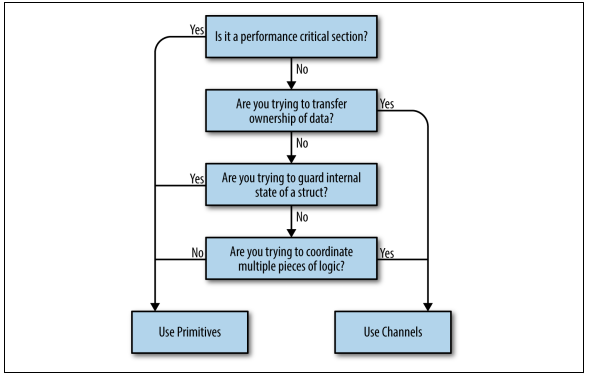
\includegraphics[width=0.7\textwidth]{pictures/ConcurrencyApproachChoose.png}
  \end{figure}

\end{frame}

\begin{frame}[fragile]
  \frametitle{Выбор подхода к организации конкурентности}
    \say{
      Regarding mutexes, the sync package implements them, but we hope Go programming style will encourage people to try higher-level techniques. In particular, consider structuring your program so that only one goroutine at a time is ever responsible for a particular piece of data.
      Do not communicate by sharing memory. Instead, share memory by communicating.
    }
\end{frame}


\begin{frame}[fragile]
	\frametitle{Заключение}
    \begin{itemize}
      \item Golang предлагает удобный подход к организации конкурентности, основанный на CSP
      \item Выполнение функций происходит в горутинах, которые размещаются на зеленых потоках
      \item Несмотря на все преимущества, в некоторых ситуациях не обойтись без классических примитив
    \end{itemize}

\end{frame}

% \begin{frame}
% 	\frametitle{Список использованных источников}
%   \printbibliography[title=Список использованных источников] % Автособираемый список литературы
% \end{frame}
\end{document}
